\section{Solar Energy}
\label{sec:SolarEnergy}

In previous sections we have seen the importance of an increase in renewable 
energy generation in order to reach climate goals. In the previous section we 
concentrated on wind power, in this one we will look at solar power. \\

Near the beginning of the course we noted that \gls{TSI} at \gls{TOA} is 
$\sim$ 1360 W/m$^2$, which if averaged over the whole Earth is $\sim$ 240 W/m$^2$
when accounting for \hyperlink{glo:albedo}{albedo}, and \textbf{in total 120 PW}
(global electricity consumption is $\sim$ 3 TW, i.e. much smaller). For these
figures, we assumed that there is no atmospheric absorption or scattering in
\gls{SW}. Remember of course that this is not quite the case - \gls{SW} is mostly
unaffected by the atmosphere but not fully. See fig \ref{fig:transmitted_radiation} \\

Let's examine this assumption a bit more closely. As per section \ref{sec:opticaldepth},
we had a definition of optical depth, in that case just for an absorbing atmosphere.

It is apparent as per fig \ref{fig:transmitted_radiation} that the atmosphere is
not just absorbing but also scattering, especially in the \gls{SW}. As a result we
will modify the definition for optical depth to replace the mass absorption 
coefficient for the \textbf{mass extinction coefficient} $\kappa_{\text{e}\lambda}$:
$$
\boxed{
    \tau_\lambda = \int_0^z \kappa_{\text{e}\lambda}(z) \rho_\text{a}(z) dz
}
\quad \text{where} \quad \kappa_{\text{e}\lambda} = \kappa_{\text{a}\lambda} + 
\kappa_{\text{s}\lambda}
$$
so the solar radiation reaching the surface becomes:
$$
I_{\text{surface}} = I_{\text{TOA}} e^{-\tau_\lambda} 
$$
so it becomes aparent that \textbf{path length} and therefore how much atmosphere
is interacting with the sunlight before reaching the surface is important in 
determining how much of it will be available at the surface. 

\noindent Before moving on, we must first define some concepts that will allow
us to progress. \\


\subsection{Some Definitions}
\label{sec:solar_definitions}

\noindent To account for path length, for solar energy applications we will often
encounter the concept of \textbf{air mass} (AM). The concept of air mass is a way to
quantify the amount of atmospheric matter (such as air molecules, aerosols, etc.)
that sunlight must traverse before it reaches the Earth's surface.
This path length of sunlight through the atmosphere is directly related to the 
amount of scattering and absorption the sunlight undergoes, which impacts its 
intensity by the time it reaches the surface.

The AM is defined as the ratio of the actual path length that sunlight travels 
through the Earth's atmosphere relative to the path length it would travel if 
the sun were directly overhead, i.e. at zenith. At zenith, sunlight travels the
shortest possible path through the atmosphere, and so this path length serves 
as our baseline (AM=1) for defining air mass. We define AM mathematically as:

$$
\boxed{
    \text{AM} = \sec (\theta_z) \quad \implies \quad I_{\text{surface}} =
    I_{\text{TOA}} e^{-\tau_\lambda \sec (\theta_z)}
}
$$
note that an air mass of 0 implies extra-terrestrial, \gls{TOA} solar irradiance
at the surface, i.e. no atmosphere.

\noindent A useful number for air mass is 1.5, which is the average air mass
at a latitude in a "temperate climate" $\sim$ 42$^\circ$ latitude (e.g. Barcelona).
This is useful since population tends to be closer to latitudes like these rather 
than the equatior or poles.\\

\noindent In the above equation we used $\theta_z$ to denote the \textbf{solar
zenith angle}, this is the angle between the direction of
the sun and the vertical (zenith direction). When the sun is directly overhead,
$\theta_z = 0$ and the air mass is 1. As the sun moves away from zenith, $\theta_z$
increases, and the sunlight has to traverse a longer path through the atmosphere,
thus increasing the air mass.\\

\noindent Total solar radiation at the surface can be broken down into two 
components: \textbf{direct} and \textbf{diffuse} radiation. 

\textbf{Direct Radiation}: This is the portion of solar radiation that comes 
straight from the direction of the Sun without undergoing any kind of scattering
or reflection. It follows a direct path from the Sun to the Earth's surface. 
This is of special interest to technologies like concentrating photovoltaics 
(CPV), which work best with direct sunlight (they use concentrating optics so
they track the sun).

\textbf{Diffuse Radiation}: This is the portion of solar radiation that has been
scattered in various directions by molecules, aerosols, and clouds in the 
Earth's atmosphere. Instead of coming from a single direction, like the Sun, 
diffuse radiation comes from multiple directions. This scattered light reaches
the Earth's surface from different angles and is important for standard 
photovoltaic (\gls{PV}) panels which can absorb sunlight from various directions (these
tend to be fixed so don't track the sun). \\

\noindent The following two terms are not crucial to know, but can be useful for a better 
understanding of the topic and its literature.

The term \textbf{global radiation} can sometimes cause confusion, as it might suggest 
something related to the entire globe. However, "global" radiation
simply refers to the total amount of solar radiation reaching a specific location
on Earth's surface, i.e., it's the sum of direct and diffuse radiation at said point.

Another term that might appear is \textbf{Direct Normal Irradiance} (DNI). 
This refers to the amount of solar radiation received per unit area by a surface 
that is always held perpendicular (or normal) to the rays that come in a straight 
line from the direction of the sun. This is particularly relevant for solar 
concentrator systems, which aim to maximize their exposure to direct radiation.

\subsection{Photovoltaic Fundamentals}
\label{sec:PV_fundamentals}

\noindent A number of further concepts are introduced in Lecture 14b, most of which
are not crucial to know for the exam. Here follows a brief summary of the most
important ones.\\

\textbf{Solar Materials}: Different materials have different uses when it comes to 
harnessing solar energy. For solar \textbf{thermal} applications, metals or black solids 
are often used because they are excellent at absorbing sunlight and converting 
it into heat. For solar chemical applications, plants are used in processes like 
photosynthesis, where sunlight is used to convert carbon dioxide and water into 
glucose and oxygen. Sometimes other chemicals are used for solar chemical
processes as well, such as in the production of hydrogen from water using
photoelectrochemical (PEC) cells. \\

\textbf{Photovoltaics}: Photovoltaic (\gls{PV}) materials are used in solar panels to convert 
sunlight directly into electricity. The key material in PV cells is a semiconductor, 
often silicon, which is 'doped' with impurities to create a so-called p-n junction 
with properties favorable for solar energy conversion. The band-gap of this 
semiconductor material is crucial - it must be suitable to absorb the energy from 
incoming solar photons, which can then excite electrons across the band-gap, 
creating an electric charge.\\

\noindent The band gap is the energy difference between the valence band (where electrons 
are normally located) and the conduction band (a higher energy level where 
electrons can move freely). When a photon with energy equal to or greater than 
the band gap hits the PV cell, it can excite an electron from the valence band 
to the conduction band, creating an electron-hole pair. The `size' of the band gap
greatly affects the performance of the PV cell. A large band gap will be excited by
high energy photons and will produce a high voltage, as they leave behind a hole
in the valence band and there is a large difference between the two (potential 
difference). However, a large band gap will not be excited by as many electrons
(the lower energy ones, higher wavelength) so the current of such cell will be lower.\\

\textbf{Photogenerated Charges}: Once the solar photons have been absorbed and the 
electrons are excited across the band-gap, these photogenerated charges 
(electron-hole pairs) need to be separated to prevent them from simply recombining. 
The p-n junction and an associated electric field help in this charge separation. 
Asymmetric contacts made to an external circuit then allow these charges to flow 
as an electric current.\\

\textbf{Power and Efficiency}: The power produced by a PV cell is the product of the 
photovoltage (the voltage generated by the photovoltaic effect) and the 
photocurrent (the current generated by the separated charges). The maximum power 
point of a cell is where the product of the photovoltage and photocurrent is 
greatest. The power conversion efficiency of a PV cell, meanwhile, is the ratio 
of the power (or power per unit area) that is converted into useful work 
(electricity), divided by the incident power (or irradiance) from the sun. 
Consistency in units is crucial when calculating efficiency.\\

% A graph showing voltage, current and power curves for a PV cell. Y axis is AU,
% X axis i band gap energy. The curves are labelled 
\begin{figure}[h]
    \centering
    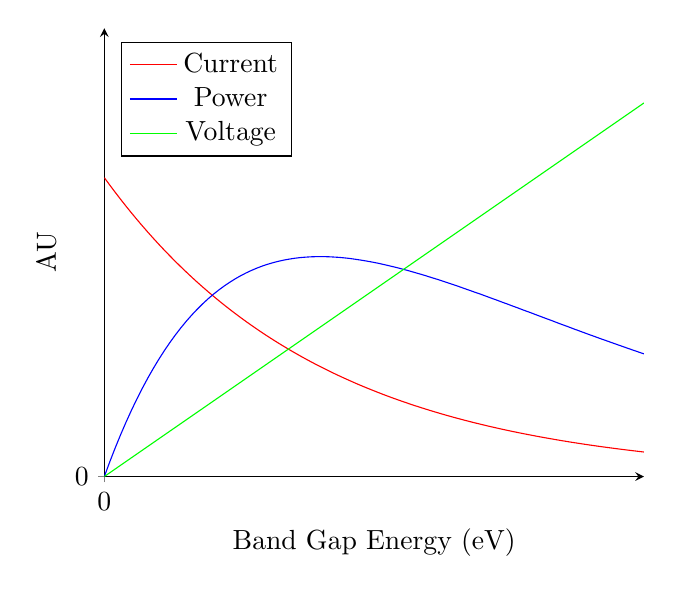
\begin{tikzpicture}
        \begin{axis}[
            axis lines = left,
            xlabel = {Band Gap Energy (eV)},
            ylabel = {AU},
            xmin = 0, xmax = 2.5,
            ymin = 0, ymax = 1.5,
            xtick={0},
            ytick={0},
            legend pos = north west,
        ]
        %Current curve
        \addplot [
            domain=0:2.5, 
            samples=100, 
            color=red,
        ]
        {exp(-x)};
        \addlegendentry{Current}
        %Power curve
        \addplot [
            domain=0:2.5, 
            samples=100, 
            color=blue,
            ]
            {2*x * exp(-x)};
        \addlegendentry{Power}
        %Voltage curve
        \addplot [
            domain=0:2.5, 
            samples=100, 
            color=green,
            ]
            {0.5*x};
        \addlegendentry{Voltage}
        \end{axis}
    \end{tikzpicture}
    \caption{Current, voltage and power curves for different band gaps. Note
    that these are estimates and not to scale.}
    \label{fig:SQ_curves}
\end{figure}


\subsection{PV Technology}
\label{sec:PV_technology}

In the lecture a number of PV technologies, each with their advantages/drawbacks
were introduced. Here follows a summary of the most important ones.\\

\textbf{Single-Junction Silicon Cells}: These are the most commonly used type of 
PV cell and are typically composed of monocrystalline or polycrystalline silicon. 
They rely on a single semiconductor material (silicon) with a specific band gap. 
This restricts the range of light wavelengths that can be absorbed and turned 
into electrical energy, hence limiting the maximum theoretical efficiency to 
about 33.7\% under standard test conditions\footnote{Said standard test conditions
try to replicate what the cell would experience under 1.5 SM, i.e. 1000 W/m$^2$
and a particular frequency spectrum. This spectrum can be found online but all that
is worth knowing is that it tries to replicate real-world conditions and that it
is normalised for 1000 W/m$^2$.} (known as the Shockley-Queisser 
limit). In practice, the efficiencies achieved are usually around 15-20\%, with 
the highest efficiencies nearing 26\%.

\textbf{Multi-Junction Cells}: These PV cells are composed of multiple layers, 
each made from different semiconductor materials with different band gaps. This 
allows the cell to absorb a broader range of light wavelengths, enhancing its 
efficiency. Each layer in the multi-junction cell is designed to absorb a 
specific range of the solar spectrum, allowing it to capture more of the 
incoming solar energy than a single-junction cell could. As a result, 
multi-junction cells can achieve efficiencies approaching 50\%. However, they 
are also more complex and expensive to manufacture.

\textbf{Alternative Material-Based Cells}: These are a diverse group of emerging 
PV technologies that use materials other than traditional semiconductors. This 
includes organic (plastic) solar cells, dye-sensitized solar cells, and 
perovskite solar cells. These technologies offer the potential for lower costs 
and more flexible applications, but they currently face challenges related to 
efficiency, stability, and scaling.
